
\chapter{Discrete Resonance Spectrum}
\label{chap:resonances}
The discrete resonances are the input information for an idealized model of auditory receptive fields, and a proxy for the information that is received by auditory cortex from the cochlea. A resonance produces, as described by \textcite{homer_modelling_2023}, a neural oscillation that damps in a short period of time. This method is an enhancement in the representation, analysis, and processing of intricate non-stationary auditory signals, outperforming the standard Fourier Transform with orthogonal basis in terms of precision due to nonlinearity. We will start with a mathematical description of discrete resonances and weave afterward some seemingly diverse mathematical topics together for the derivation of the Fast Padé Transform. Finally, the benefits of a non-orthogonal basis in a Hilbert space will be demonstrated.


\section{Discrete Resonances in Time Domain}

As with Fourier analysis a time-domain signal can be decomposed in different sines and cosines, a signal can also be decomposed in a linear combination of $K$ complex oscillators ("resonances"). 
These time-domain signals are defined as follows:

\begin{equation}
    x(t) = \sum^K_{k=1} d_ke^{-i\omega_kt} 
    \; \; \; \; \; \; \; \; \; \; \; \; \; \; 
    d_k, \omega_k \in \mathbb{C} .
\end{equation}

\begin{marginfigure}
\centering
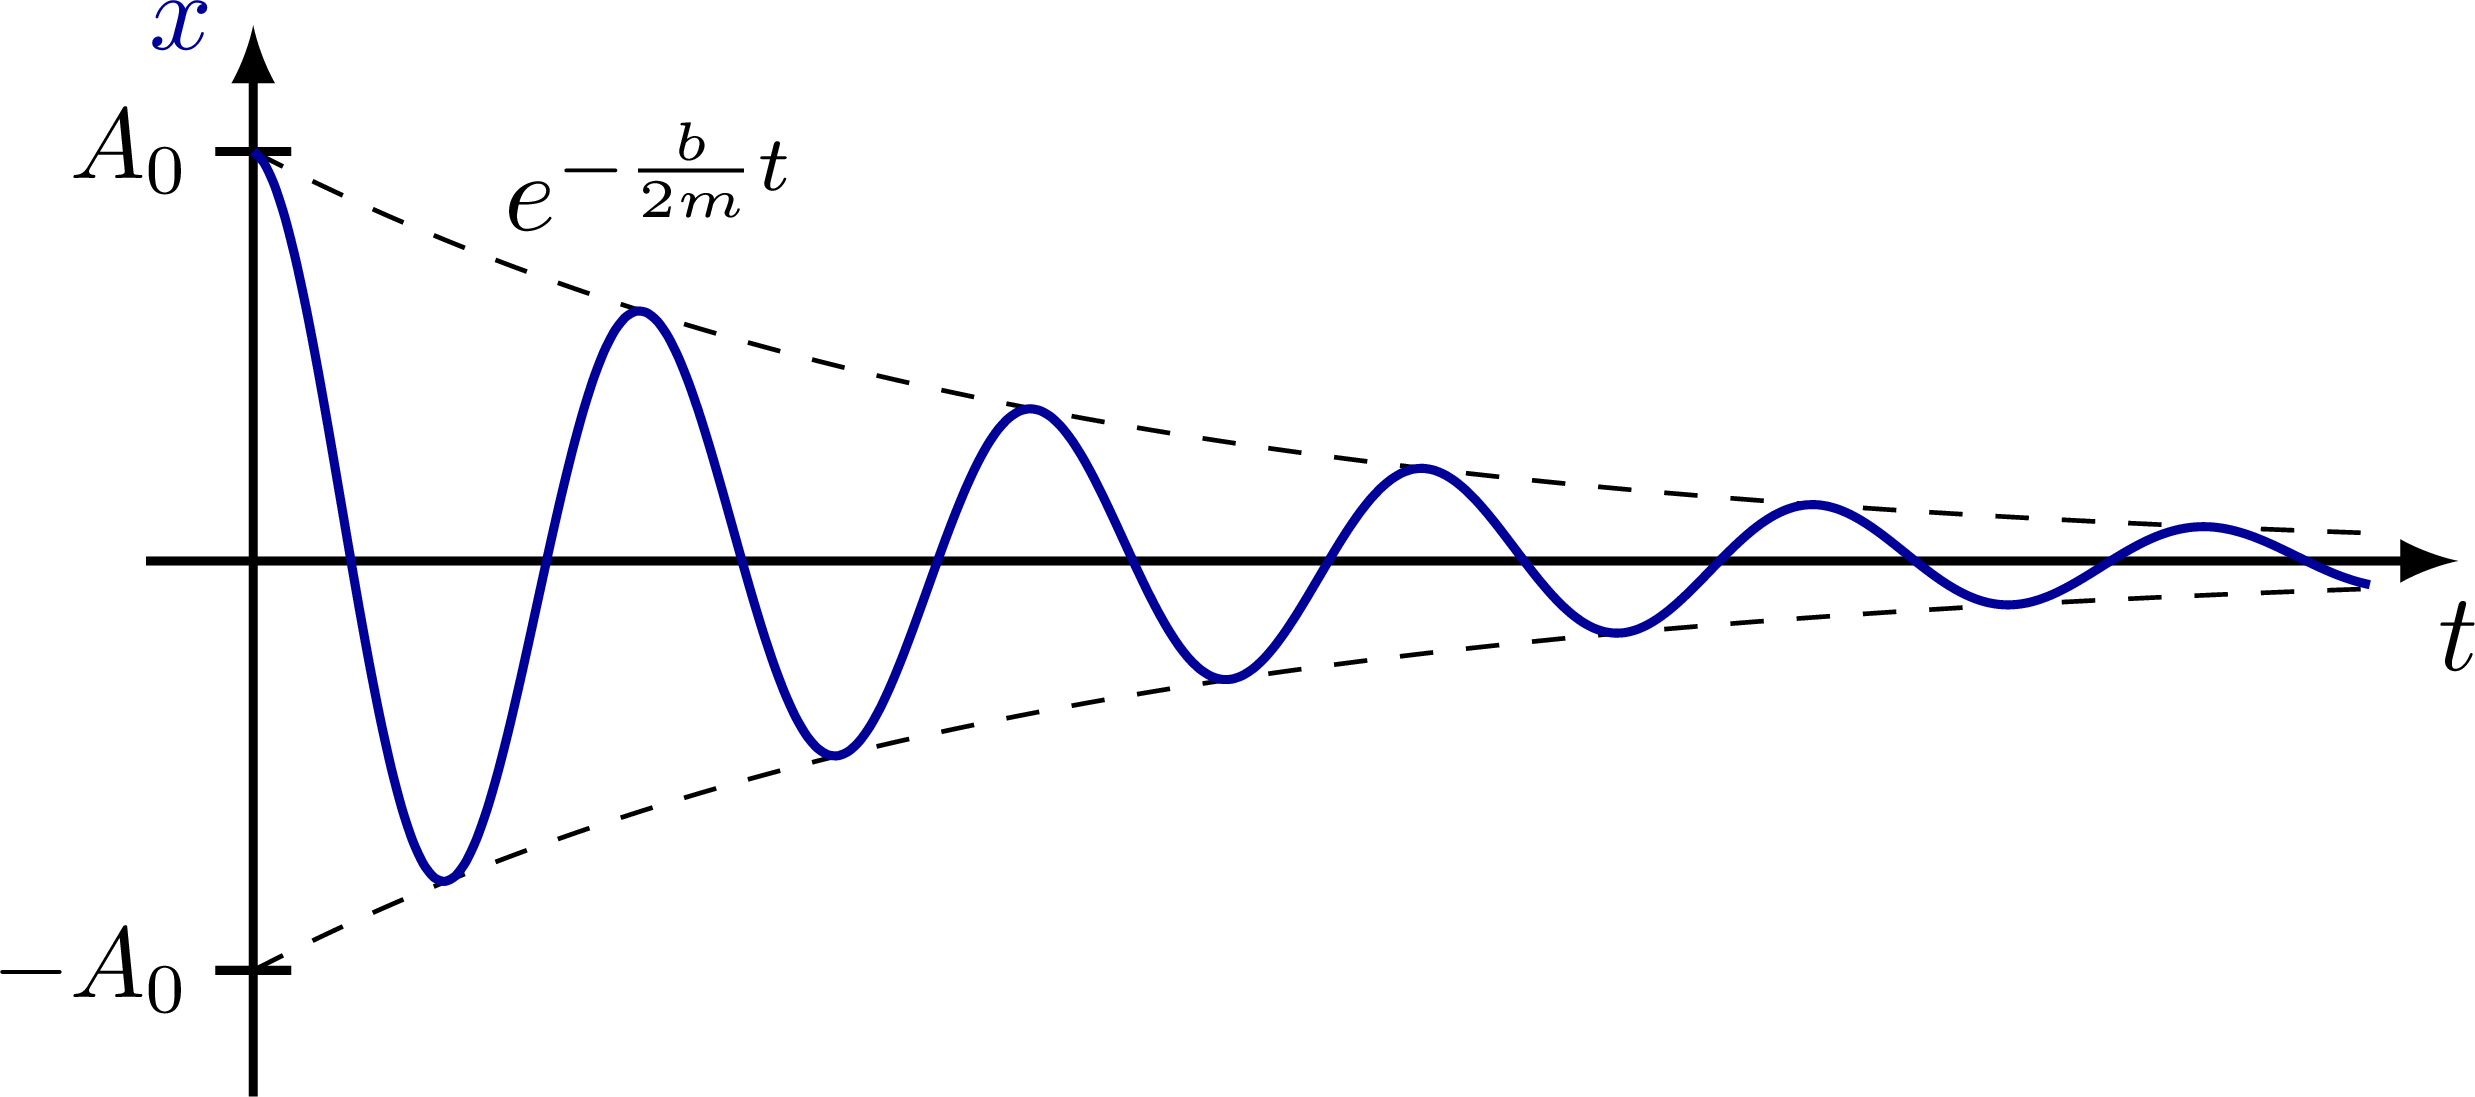
\includegraphics[width=0.9\linewidth]{images/resonances/dynamics_oscillator.png}
\caption{Visualization of the real part of a resonance with an exponential decay factor as an envelop (\cite{neutelings_harmonic_2021}).}
\label{dampedHarmonic} \vspace{3cm}
\end{marginfigure}

Signal $x$ is formed by a summation of different complex resonances with $d_k$ the initial complex amplitude of the oscillator and a rotating vector $e^{-i\omega_kt}$, dependent on the complex frequency $\omega_k$. It might seem illogical to see the notation of a continuous signal for discrete resonances (i.e., $x(t)$ instead of $x[n]$). We will leave the details behind this formulation beside, the important thing is to know that it is based on the Continuous Fourier Transform, and will only be discretized in the actual implementation.

Just to prevent confusion with the previous chapter: the definition of resonances describes a time-signal that is decomposed in damped or driven oscillators, just like Fourier series did for stationary signals. In resonances, a fourth dimension is added, containing the decay. In a 3D representation, the following visualization in Figure \ref{fig:resonace3D} of a resonance can give a more intuitive feeling for its appearance. The decay can be observed as the complex exponential function in Figure \ref{dampedHarmonic}.


\begin{figure}[ht]
    \centering
    \adjustbox{width=1\linewidth}{\resonance{}}
    \vspace{0.3cm}
    \caption{A visual representation of a resonance in 3D.}
    \label{fig:resonace3D}
\end{figure}

The complex frequency $\omega_k$ consists of a real and imaginary part, namely the frequency of the resonance $\phi_k$ and the rate of decay $\gamma_k$ as a complex part: $\omega_k = \phi_k +i \gamma_k$. A short mathematical interpretation illustrates the intuition behind this formulation: 

\begin{marginfigure}
\centering
\includesvg[width=0.9\linewidth]{images/resonances/resonanceComplex.svg}
\caption{A discrete resonance with the complex part visualized with dotted lines and the real part with the continuous line (\cite{homer_modelling_2023}).}
\label{resonanceComplex} 
\vspace{3cm}
\end{marginfigure}

\begin{equation}
\begin{split}
e^{-i\omega_kt} &= e^{-i(\phi_k + i\gamma_k)t}  \\
&= e^{-i\phi_k t + \gamma_k t} \\
&= e^{\gamma_k t}e^{-i \phi_k t} \\
&= e^{\gamma_k t} [\cos(\phi_k t)-i \sin(\phi_k t)] \\
&= e^{\gamma_k t} [\cos(\phi_k t)+i \sin(\phi_k t)]^*
\end{split}
\end{equation}

$\gamma_k$ describes the decay of the resonance, and the sine and cosine terms are a representation of the oscillatory behavior and denote the frequency.  Visually, one can think of it as decayed or augmented sine waves. 
Furthermore, $d_k$ can be rewritten as $|d_k|e^{i\psi_kt}$, with $\psi_k$ denoting the initial phase of the oscillator. The absolute value of the amplitude is the polar representation of $d_k$.
\begin{equation}
    x[t] = \sum^K_{k=1} |d_k|e^{i\psi_kt} e^{-i(\phi_k + i \gamma _k)t}  
    \; \; \; \; \; \; \; \; \; \; \; \; \; \;
    |d_k|, \psi_k, \phi_k, \gamma_k \in \mathbb{R}
\end{equation}



\section{Discrete Resonances in Frequency Domain}


The Fourier transform is a tool for performing spectral analysis of time-domain signals. It is defined with respect to frequency $\phi$. Here, the oscillatory signal is represented in the frequency domain:
\begin{equation}
    X(\phi) = \frac{i}{\sqrt{2 \pi}} \sum^K_{k=1} \frac{d_k}{\phi - \omega_k} = \frac{i}{\sqrt{2 \pi}} \sum^K_{k=1} \frac{|d_k| e^{i\psi_k}}{\phi - (\phi_k + i \gamma_k)}.
\end{equation}
The absolute value of the amplitude $d_k$ corresponds in the frequency domain to the size of the resonance peak. Frequency $\phi_k$ defines the location of the resonance peak, and decay $\gamma_k$ influences the width and polarity of the resonance peak in the frequency domain. Here, again, $\psi_k$ is the initial phase of the oscillator. In the frequency domain, it has an effect on altering the angle of the rotating vector, thus the cotangent of the angle: $\Re[f(\phi)]/\Im[f(\phi)]$. 

\begin{marginfigure}
\centering
\includesvg[width=0.9\linewidth]{images/resonances/resonanceFreqSpec.svg}
\caption{A discrete resonance in the frequency domain (\cite{homer_modelling_2023}).}
\label{resonanceFreqSpec} 
\end{marginfigure}

\section{The Fast Padé Transform (FPT)}

In section \ref{sec:FFT}, we briefly discussed the Fast Fourier Transform. The power for finding the coefficients hides in the specific selection and evaluation of complex numbers sitting evenly spaced on the unit circle, or, in other words, due to the restriction of having orthogonal bases in a Hilbert Space. 

However, when the complex numbers are not evenly spaced, and not even necessarily on the unit circle (which is the case for discrete resonances), it becomes a quite expensive operation to find those coefficients. Therefore, Steven Homer (personal communication, 2023) applied The Fast Padé Transform (\cite{belkic_signal_2019}) on resonances to estimate the spectral density function of a time series signal, which is a distribution of the power of a signal across different frequencies. The Fast Padé Transform itself is a numerical algorithm for approximating the power series expansion of a function in a given interval. It is a fast and efficient and can compute the coefficients of a Padé approximant, which is a rational function that interpolates the power series expansion of a function


\subsection{Preliminary Knowledge}
We will begin by refreshing key concepts from linear algebra. This primer will help establish a solid foundation for understanding the mathematical derivation of the Fast Padé Transform.

\begin{definition}[Generating function]
A generating function $G(x)$ encodes an infinite sequence of numbers by treating them as coefficients of a formal power series. 
\end{definition}
A simple example of a generating function is the encoding of even numbers with 

\begin{equation}
    G(x) = \frac{2x}{(1-x)^2}, 
\end{equation}

which will generate the sequence of even numbers $\{0, 2, 4, 6, 8, ...\}$. 

\begin{definition}[Constant-recursive sequence]
A constant-recursive sequence is an infinite sequence of numbers, where each number in the sequence is equal to a fixed linear combination of one or more of its immediate predecessors.
\end{definition}
This feature will be important in the further derivation, since the sequence is constant recursive, this will allow us to define analytic functions in a Hilbert space.

% \begin{definition}[Sequence versus series]
% A sequence orders the numbers in a certain order, when series refers to the summation of the terms.
% \end{definition}

% \begin{definition}[Closed-form expression]
% A mathematical expression that uses a finite number of standard operations.
% \end{definition}

% \begin{definition}[The fundamental theorem of algebra]
% The fundamental theorem of algebra states that every non-constant single-variable polynomial with complex coefficients has at least one complex root."
% \end{definition}


\subsection{Mathematical Derivation}
We will now discuss the rough structure of a mathematical derivation for the Fast Padé Transform originating from \textcite{belkic_signal_2019} and applied to the resonance spectrum by Steven Homer (personal communication, 2023).

Assume the ordinary generation function $G$ of the infinite constant-recursive sequence of numbers ($c_n$):
\begin{equation}
	G(c_n,z) = \sum_{n=0}^\infty c_n z^{n}.
\end{equation}
$z$ denotes a coordinate in polar representation (i.e., $e^{-iw_kt}$). 

By definition, a \textit{formal} power series does not have to converge, but since this generating function is defined to be an analytic function in a Hilbert Space, it means that it has a convergent power series expansion. The goal of the derivation is to come define a closed-form expression that can be evaluated and makes the definition valuable. Assuming that $c_n$ is constant-recursive sequence, the generative function can be rewritten as 

\begin{equation}
	G(c_n,z^{-1}) = \sum^\infty_{n=0} c_n z^{-n} =\frac{\sum\limits_{k=0}^{K-1}p^-_kz^{-K}}{1+\sum\limits_{k=1}^{K}q^-_kz^{-K}} \left( \frac{z^K}{z^K} \right)
\end{equation}

Which is a Padé approximate by definition. Note that, for the sake of math, a multiplicative inverse of the complex number $z$ was used. The modification to the negative angle does not change anything about the real value of the signal, since a real number is equal to a complex number (no matter positive or negative) with its imaginary part equal to zero. The negative annotation at the coefficients was introduced to denote that they are a coordinate in the negative domain. After the derivation, it returns to the positive domain. The derived generic function can be rewritten as




\begin{equation}
	\sum^\infty_{n=0} c_n z^{-n} = \frac{\sum\limits^K_{k=1} p_k z^k}{1+\sum\limits^K_{k=1}q_kz^k}
 %z \frac{p_{k-1}^+(z)}{q_k^+(z)}
\end{equation}

This equation is solvable by deriving this equation with respect to the variable $z$. By introducing the initial complex amplitude $d_k$, the equality can be rewritten as

\begin{equation}
    \sum^K_{k=1} \frac{d_k}{1-(\frac{z_k}{z})}
\end{equation}


For a full derivation, please read \textcite{belkic_signal_2019}, page 65-77). This form looks exactly as a geometric series $\sum^\infty_{n=0}ar^n=\frac{a}{1-r}$, with $|r| < 1$ and thus if the following inequality holds: $|\frac{z_k}{z}|<1$, the equality can be written as

\begin{equation}
 \sum^K_{k=1} d_k \sum^\infty_{n=0}(\frac{z_k}{z})^n.
\end{equation}
Therefore,
\begin{equation}
    c_n = \sum^K_{n=1} d_k z_k^n.
\end{equation}

Notice that $z_k$ represents the complex plane. The derived summation represents a function in $n$. If the signal is a simple cosine, then it moves around the unit circle when n increases. In the case that the frequency is complex, and the decay is non-zero, the coordinates will fall inside or outside the unit circle. In other words, $c_n$ can be expressed as a sum of oscillators. Solving this equation for $d_k$ and $z_k$ is exactly what the FPT does in a certain interval, i.e., rectangular window, defined as following:

\begin{equation}
    \sum^\infty_{n=0} c_n z^{-n} - \sum^\infty_{n=N} c_n z^{-n}
\end{equation}
Solving the equation by substituting it with the derivation we had before, gives us
\begin{equation}
    \sum^{N-1}_{n=0} c_n z^{-n} = \frac{\sum\limits_{k=1}^K p_k z^{k}+\sum\limits_{k=1}^K r_k z^{k-N}}{1+\sum\limits_{k=1}^K q_kz^k}
\end{equation}
For a window function where $p$ and $r$ represents the coefficients at the left and right side of the window. which is exactly the FPT (can also be seen as a convolution). Essentially, this derivation allows us to find the $c_n$'s and $z$, and therefore the oscillators. And since K = N/2, there is a unique solution.

\begin{marginfigure}
\centering
\includesvg[width=0.9\linewidth]{images/resonances/resonance_circle.svg}
\caption{A pole-zero diagram consisting of distinct points that are not uniformly distributed due to the non-orthogonal bases and are no longer located on a unit circle due to the complex frequency $\omega_k$.}
\label{resonanceCircle} \vspace{3cm}
\end{marginfigure}

\subsubsection{Non-Orthogonal Bases in a Hilbert Space}

Although the usage of orthogonal bases ensures efficient computation and a simple representation, using a collection of non-orthogonal basis functions can be advantageous in some cases, such as in the Hilbert Space of Resonances. The non-orthogonal bases allow us to have non-evenly spaced frequencies $\gamma_k$, which is a sequence of numbers. By gaining more freedom with the placement of the frequencies in this space, the frequencies of a signal can be found more precise without limiting itself to a sample rate, as illustrated in Figure \ref{resonanceCircle}, and a bigger space in the complex plane can be explored.

Consider now the normalized sequence of signals




\begin{equation}
    \phi_k(t) = e^{i \omega_k t}  \; \; \; \; \; \; \; \; , k \in \mathbf{Z}.
\end{equation}

Here, $\omega_k$ is a sequence of numbers and if  $\omega_k$ = k, we obtain the classical Fourier series basis, with $\phi_k$ an orthogonal basis. 
However, if $\omega_k$ is not an integer multiple, the signals are not orthogonal (\cite{romberg_ece_2016}). Since $\omega_k$ is a complex function in our application of resonances (a complex frequency that makes the sinusoidal decay), we do not have evenly spaced points anymore in the discretization of the formula, as is shown in Figure \ref{resonanceCircle}.
The reason why a signal can equivalently be decomposed into resonances, as Fourier analysis does with sines and cosines, is because
\begin{marginfigure}
\centering
\vspace*{-7cm}
\includesvg[pretex=\fontsize{4pt}{6pt}, width=0.9\linewidth]{images/fftvsfpt/stft_a4_top.svg}
\label{topview_stft} 
\end{marginfigure}
\begin{marginfigure}
\vspace*{-1.6cm}
\centering
\includesvg[pretex=\fontsize{8pt}{10pt}, width=0.9\linewidth]{images/fftvsfpt/stft_a4.svg}
\caption{A filtered Fourier spectrogram showing the fundamental A4 and its overtones performed by a flute.} 
\label{fourierSpectrogram} 
\end{marginfigure}
\begin{marginfigure}
\centering
\vspace*{1.2cm}
\includesvg[pretex=\fontsize{4pt}{6pt}, width=0.9\linewidth]{images/fftvsfpt/fpt_a4_top.svg}
\label{topview_fpt} 
\end{marginfigure}
\begin{marginfigure}
\centering
\includesvg[pretex=\fontsize{8pt}{10pt}, width=0.9\linewidth]{images/fftvsfpt/fpt_a4.svg}
\caption{A filtered resonance spectrogram representing the same fundamental A4 and its overtones performed by a flute. Note the high precision of this method.}
\label{resonanceSpectrogram} 
\end{marginfigure}
\begin{equation}
    e^{\gamma t} cos(\phi_k t) = \frac{1}{2}( e^{i (\phi_k + i \gamma_k) t} +  e^{-i (\phi_k - i \gamma_k) t}).
\end{equation}
Summarized, $\braket{f|g} = 0$ is not required to be true from an algebraic point of view and the complex frequency with a decaying factor uses non-orthogonal basis.




\section{Towards higher Precision with Non-Orthogonal Bases in a Hilbert Space}
\label{sec:nonorthogonalBases}

Due to the non-orthogonal property of the Fast Padé Transform, the size of each frequency bin in a time slice is varying with respect to the parameters of a resonance. This has enormous advantages in terms of precision when performing spectral analysis. Figures \ref{fourierSpectrogram} and \ref{resonanceSpectrogram} provide a visual demonstration of the fundamental difference between the widely used Short Time Fourier transform and the Fast Padé Transform with a synthetic audio recording of a flute performing the musical note A4. The visualized signals were filtered on power and frequency for the purpose of simple visualization of the main difference between the two methods. The frequency was set in a range between 0 and 2000 since the fundamental frequency and its observable harmonics generally lay between this range (\cite{huang_resonance-based_2017}). Resonances with a relatively small power were also removed from both plots.
In Figure \ref{fourierSpectrogram}, the resolution of the time and frequency domains are fixed and bound with the STFT, and due to that, the signal is estimated with a division over several nearest frequency bins, bounded by Heisenberg's uncertainty principle (\cite{folland_uncertainty_1997}). However, due to the non-orthogonal requirements of the basis, the size of frequency bins may vary and a more precise estimation of the frequency components can be achieved.


 \section{Extracting Attributes from the Discrete Resonance Spectrum}
 \subsection{Dynamic Resonances}
 The dynamic resonance is a non-explicitly documented technique (Homer, personal communication, 2023), wherein different distance metrics were used to combine two resonances in consecutive slices with each other. The six distance measures were defined as following: frequency distance, harmonic mean of the $d_k$ and $w_k$ coefficients, residue of the product of the resonances, residue of the product of the resonances weighted by power, residue of the product of the resonances multiplied by the spectra transference function and residue of the product of the resonances multiplied by the spectra transference function weighted by power.

A dynamic resonance is a relation of the distance metric $d$ defined as following:



\begin{definition}[dynamic resonance]
Let $S_x$ and $S_{x+1}$ be non-empty consecutive slices in a spectrogram $S$ with distinct resonances, and let $d(i, j)$ be a distance function defined for all pairs $(i, j)$ representing those resonances, such that $i \in S_x$ and $j \in S_{x+1}$. We define the relation $R$ as follows: 

\begin{equation}
    \forall i \in S_x, \exists j \in S_{x+1}: d(i,j) \leq d(i,k) \; \; \;  \; \; \forall k \in S_{x+1} \smallsetminus \{j\}.
\end{equation}

\end{definition}

\begin{marginfigure}
\centering
\includesvg[pretex=\fontsize{8pt}{10pt}, width=0.8\linewidth]{images/cluster/measurement.svg}
\vspace{0.1cm}
\caption{Two consecutive slices $S_x$ and $s_{x+1}$ and the relation between two resonances measured with a distance function $d$.}
\label{distanceMeasurement} 
\end{marginfigure}

 \begin{marginfigure}
    \centering
    \vspace{2cm}
    \includesvg[ width=1\linewidth]{images/cluster/dynamicResonances.svg}
    \caption{Dynamic Resonance spectrum.}
    \label{fig:DynamicResonance}
\end{marginfigure}

Due to the slow computational speed of Python and excessive usage of loops, his approach worked significantly slower than our density based approach. However, the insight of using other distance measurements than the Euclidean for the definition of distance inspired us to measure similarity between resonances with the following definition:
 

\begin{equation}
    \cos (d_{jk}) = \frac{\Re \left[\frac{d_jd_k}{w_j-w_k}\right]}{\frac{|d_j|^2}{\gamma_j}\frac{|d_k|^2}{\gamma_k}}
\end{equation}

After implementing and evaluating this approach, the distance measurement based on similarity of resonances did not contribute to a better clustering. However, it can serve as an inspiration for using other distance measurements in future work to extract more features from the data.


\section{Summary}
We started this chapter with the definition of the discrete resonances in the time and frequency domain and summarized the proof of the Fast Padé Transform, which is a discrete convolution of the coefficients $c_n$ with the coefficients $q_k$, yielding the coefficients $p_k$ and $r_k$ and zeros. We showed that the main difference with Discrete Fourier Transform is the use of a non-orthogonal basis in a Hilbert Space. We introduced \textit{dynamic resonances} as a novel method for grouping resonances. However, it requires high computational power and therefore, we will introduce a cognitive-based method for cluster analysis for the extraction of musical structures from the discrete resonance spectrum.



